\section{Case Study: CookieCAD}
\label{sec:CS}

As a running example for illustrative purpose, we take a very simplified variant of 
Computer-Aided Design (\textsc{Cad}) named CookieCAD (\textsc{CCad}). 
\textsc{CCad} aims at designing simple cookie cutters, as illustrated with a triangle shaped cookie cutter in Figure \ref{fig:CookieCAD}(a). A cookie cutter has a certain shape (like 
triangle, rectangle, star, etc.) represented by 2D geometric lines (noted 
$L$), which are specified based on the definition of points (noted $P$) placed 
on a cartesian plan (using x- and y-coordinates). Shapes must represent 
closed polygons. Shapes may share some lines (for example, defining a 
house-shaped cookie cutter by associating a triangle for the roof, placed over a 
rectangle, as shown in Figure \ref{fig:CookieCAD}(b)). Consequently, lines shall not cross each others as illustrated in Figure \ref{fig:CookieCAD}(c), which results in an \emph{invalid} cookie cutter.

\begin{figure}[t]
   \centering
   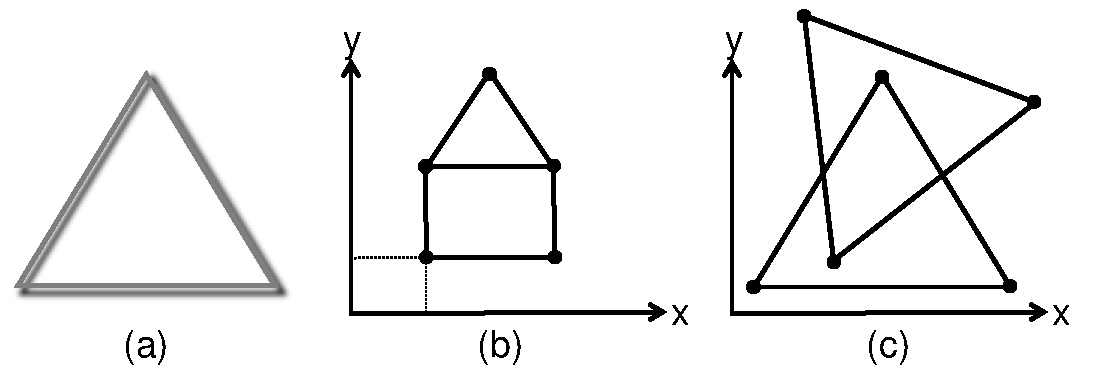
\includegraphics[width=\columnwidth]{CookieCAD.pdf}
   \caption{CookieCAD Examples: (a) A simple real-life cookie cutter. (b) A 
house-like shape sharing a line. (c) An invalid shape (due to overlaps).}%  
   \label{fig:CookieCAD}
\end{figure}

%Many engineering disciplines (civil, mechanical, electrical, among others) 
%require an \emph{a priori} \emph{design}, i.e. a kind of specification, or plan, 
%of the final object, be it a bridge, a car's clutcher, or a complex electronic 
%card. From an \textsc{Mpm} viewpoint, designs play the role of \emph{models}: 
%they abstract from the real product while still possessing interesting 
%properties, making them cheaper to produce and easier to analyse. To support 
%designers, Computer-Aided Design (\textsc{Cad}) promotes the use of computers to 
%help create, modify, and analyse designs, but also optimise against known 
%constraints from a given domain. \textsc{Cad} has significantly improved many 
%engineering disciplines by improving the designs quality and increase the 
%designers' productivity, and even becoming standard development tools for 
%disciplines like electronics. \textsc{Cad} tools allow the \emph{visually} 
%design in 2D, 3D and even 4D (adding the time dimension), based on various 
%techniques such as Finite Element Methods, thus manipulating complex 
%Differential Equations. 

%For the purpose of this introductory work, we propose the Poor-Man \textsc{Cad} 
%(abbreviated as \textsc{PCad}), a (toy) (multi-)formalism that allows designing 
%2D geometric lines (noted $L$) representing arbitrary shapes, based on the 
%definition of points (noted $P$) placed on a cartesian plan (defined by integer 
%X- and Y-coordinates). When required, lines may be colored to emphasize 
%surfaces of a shape or parts of a design. Colors (noted as $C$) are encoding as 
%RGB integer triples for simplicity. The following Definition and Example 
%provides a formal specification and a visual representation of a possible 
%design.

\begin{Definition}[\label{def:CCAD}Cookie-CAD Shapes] A \CCad-shape (or design) $s\in \CCAD$ is a set of lines. 
A \emph{line} $l \in L$ is defined as a set of exactly two points.
A \emph{point} $p\in P$ is a pair of reals.
The function $\SMapping$ maps shapes $s\in \CCAD$ to the union of points 
the lines constituting the shapes are made of.
\begin{displaymath}
   \begin{small}
      \begin{array}{rcl rcl}
         \CCAD &\eqdef& \wp(L) \\
         L     &\eqdef& \{ \{p, p'\} \;|\; p, p' \in P, p\neq p' \} \\
         P     &\eqdef& \mathbb{R} \times \mathbb{R}
      \end{array}
   \end{small}
\end{displaymath}

The semantics of a \CCad-shape is captured by the function 
$\SMapping$, that maps each shape to the points the lines constituting the 
shape is built upon. 
\begin{displaymath}
   \begin{small}
      \begin{array}{rcl}
         \SMapping & \colon & \!\!\!
            \begin{array}[t]{rcl}
               \CCAD &\to& \wp(\wp(\mathbb{R}^2)) \\
                   o &\mapsto& \lbrace \lbrace u,v\rbrace \;|\; \exists 
u,v\in \mathbb{R}.\; 
                    \forall x \leq u \leq x'. \\
& & v{=}m{*}u{+}\left(y{-}m{*}x\right), o{=}\lbrace \lbrace x, y \rbrace, \lbrace x', y' \rbrace \rbrace,
%%
            \end{array}\\
      \end{array}
   \end{small}
\end{displaymath}
\noindent 
where $m = \frac{y'-y}{x'-x}$ and w.l.o.g. $x' \geq x$.
\end{Definition}

A metamodel comprising the syntax elements of \CCAD could be as depicted in
Fig.~\ref{fig:PCAD-MM}. Here, a \CCAD drawing has a name and a set of lines, each
defined by a start point and an end point. The points between these two
points are not part of the \CCAD syntax as defined above.

\begin{figure}[t]
\centering

\includegraphics[width=0.98\columnwidth]{CCAD-MM}
\caption{A metamodel for \textsc{CCad} (cf. Def.~\ref{def:CCAD}).}
\label{fig:PCAD-MM}%
\end{figure}

As minimal activities on \textsc{CCad} designs, one shall evidently \emph{draw
lines} to create shapes, \emph{check} their validity (e.g., to prevent cookie
cutters with overlapping edges), and ultimately \emph{3D print} the cutters
from the designs.




% \subsection{Finite-State Automata}
% \label{sec:Examples-FSM}
% 
% Finite State Automata (\textsc{Fsa}), as originally defined by Moore 
% \cite{J:Moore:1956}, link states with transitions that carry a label. 
% \textsc{Fsa} describe discrete state-based computations. Many variations of 
% \textsc{Fsa} exist together with various semantics, among which the 
% ``word-accepting'' semantics is one of the most used \cite{}. 
% 
% The \UML State Machines \cite{TR:UML-2.5:2015} is the language used by many 
% tools for expressing, among other possibilities, the behaviour of a \UML 
% object. Beyond state-based computations, \UML State Machines add several new 
% concepts like hierarchical and orthogonal states, history, and the possibility 
% to interact with the environment through outputs.
% 
% \subsection{Java}
% \label{sec:Examples-Java}
% 
% Java \cite{B:Java:2019} is a modern object-oriented programming language that 
% has become widely used for a large variety of applications. 
% 
% Wegner criteria for OO \cite{Wegner:1987}
% 
% \subsection{The \textsc{Md}$\star$ Jungle of Acronyms}
% \label{sec:Examples-MD}
% 
% \cite{B:Brambilla-Cabot-Wimmer:2012}


\begin{table}[t]
   \begin{center}
      \begin{tabular}[t]{c l}
         \hline
         \multicolumn{2}{l}{$\iota_1$: State Automata ($\mathsf{SA}$)}\\
         \hline
         $\mbox{SA}_1$ & Contains the concepts of State and Transition\\
         $\mbox{SA}_2$ & Possess a Transition enabler\\
         $\mbox{SA}_3$ & Changes state when a transition is enabled\\
         \hline\hline
         \multicolumn{2}{l}{$\iota_2$: Object Orientation ($\mathsf{OO}$)}\\
         \hline
         $\mbox{OO}_1$ & Possess the concepts of Object and Class\\
         $\mbox{OO}_2$ & Objects possess a state and a set of capabilities / operations \\
         $\mbox{OO}_3$ & Possess an inheritance mechanism\\
         $\mbox{OO}_4$ & Inheritance allows to reuse operations\\
         \hline\hline
         \multicolumn{2}{l}{$\iota_3$: Computer-Aided Design ($\mathsf{CAD}$)}\\
         \hline
         $\mbox{CAD}_1$ & Comprises concepts of (2D/3D) points and lines\\
         $\mbox{CAD}_2$ & Shapes are defined by lines\\
         $\mbox{CAD}_3$ & Supports transformation into (2D/3D) products\\
         \hline
      \end{tabular}
   \end{center}
   \label{tab:Properties}
   \caption{Properties of three paradigms: State Automata ($\mathsf{SA} 
\cite{J:Moore:1956}$); Object Orientation ($\mathsf{OO} \cite{Wegner:1987}$) 
and Computer-Aided Design ($\mathsf{CAD} \cite{CAD}$)}
\end{table}
